\section{Concepto y Definiciones.}
Para introducirnos al estudio y análisis de la economía, es importante desarrollar algunos conceptos previos que permitan comprender de manera adecuada los elementos que se van a desarrollar en los siguientes párrafos así como en los posteriores capítulos. Inicialmente se puntualizará conceptos fundamentales para comprender el estudio de la economía desde una perspectiva general, es así que debemos iniciar este capitulo desarrollando el concepto de economía. \\
\subsection{Economía}
\begin{caja}[La palabra economía proviene del griego \textbf{"oikonomos"}, que significa \textit{\textbf{"el que administra una casa".}}]
	La economía se ocupa de las cuestiones que surgen en relación con la satisfacción de las necesidades de los individuos y de la sociedad. La satisfacción de necesidades materiales (alimentos, vestimenta o vivienda) y no materiales (educación, ocio, etc.) de una sociedad obliga a sus miembros a llevar a cabo determinadas actividades productivas, mediante estas se obtienen los bienes y los servicios que se necesitan, entendiendo por bien todo	medio capaz de satisfacer una necesidad tanto de los individuos como de la sociedad.
\end{caja}

Por tanto, \textbf{la economía se ocupa de la
manera en cómo la sociedad administra sus recursos escasos}\footnote{Gregory Mankiw: Principios de Economía}, con
objeto de producir diversos bienes y distribuirlos para su
consumo entre los miembros de la sociedad. En la mayoría de las sociedades los recursos se distribuyen por medio de las acciones de todos loa agentes económicos.\\

El estudio de la Economía tiene lugar bajo dos enfoques: el microeconómico y el macroeconómico. La Microeconomía estudia los comportamientos básicos de los agentes económicos individuales y la La Macroeconomía es el estudio de fenómenos agregados o globales que afectan al conjunto de la economía.

\begin{definicion}[Actividad Productiva]
	Es el proceso a través del cual la actividad del hombre transforma los insumos tales como materias primas, recursos naturales y otros insumos, con el objeto de producir bienes y servicios que se requieren para satisfacer las necesidades.
\end{definicion}	

\begin{definicion}[Economía]
	La economía es la ciencia que se ocupa del estudio sistemático de
	las actitudes humanas orientadas a administrar los recursos, que son
	escasos, con el objetivo de producir bienes y servicios y distribuirlos
	de forma tal que se satisfagan las necesidades de los individuos, las
	que son ilimitadas.
\end{definicion}

\begin{definicion}[Escasez]
	Carácter limitado de los recursos de la sociedad, esto significa que la sociedad tiene recursos limitados y, por tanto, no puede producir todos los bienes y servicios que las personas desearían tener.
\end{definicion}	

\begin{definicion}[Agentes Económicos]
	Son los sujetos que intervienen en toda actividad económica y se identifican  tres tipos de agentes: las familias, las empresas y el Estado.
\end{definicion}	




\subsection{La escasez y la elección}
La escasez debemos entenderla como la  disparidad entre deseos humanos y medios disponibles para satisfacerlos.
Los individuos tratan de cubrir inicialmente aquellas necesidades queEl capital humano son los conocimientos
y cualificaciones adquiridos por los individuos
por medio de la educación y de la experiencia. son biológicas o primitivas, esto es, las
relacionadas con la alimentación, la vivienda y la vestimenta. De igual manera, los individuos necesitan proveerse
de ciertos servicios como los de asistencia médica, educación, transporte, etc. Una vez cubiertas las anteriores necesidades, los individuos se ocupan de aquellas otras que hacen placentera la vida, si bien el nivel de cobertura de éstas dependerá del poder adquisitivo de cada individuo en particular.

\subsection{Factores Productivos}
Los factores o recursos productivos son los recursos empleados por las empresas o unidades económicas de producción para producir bienes y servicios.\\

La economía clasifica de manera tradicional los factores productivos en tres categorías:
\begin{itemize}
	\item \textbf{La tierra (o recursos naturales):} todo lo que aporta la	naturaleza al proceso productivo.
	\item \textbf{El trabajo:} el tiempo y las capacidades intelectuales	dedicadas a las actividades productivas.
	\item \textbf{El capital\footnote{En economía, a menos que se especifique lo contra	rio, el término capital significa capital físico, es decir,	máquinas y edificios, y no capital financiero.}:} los bienes duraderos no dedicados al consumo sino a producir otros bienes.
\end{itemize}

\begin{definicion}[El capital humano]
	Son los conocimientos	y cualificaciones adquiridos por los individuos
	por medio de la educación y de la experiencia.
\end{definicion}

\section{Principios de la Economía.}
El estudio de la economía tiene múltiples facetas, pero se encuentra unificado por
varias ideas fundamentales. En este capítulo estudiaremos los Diez principios de la
economía.\\

\begin{center}
	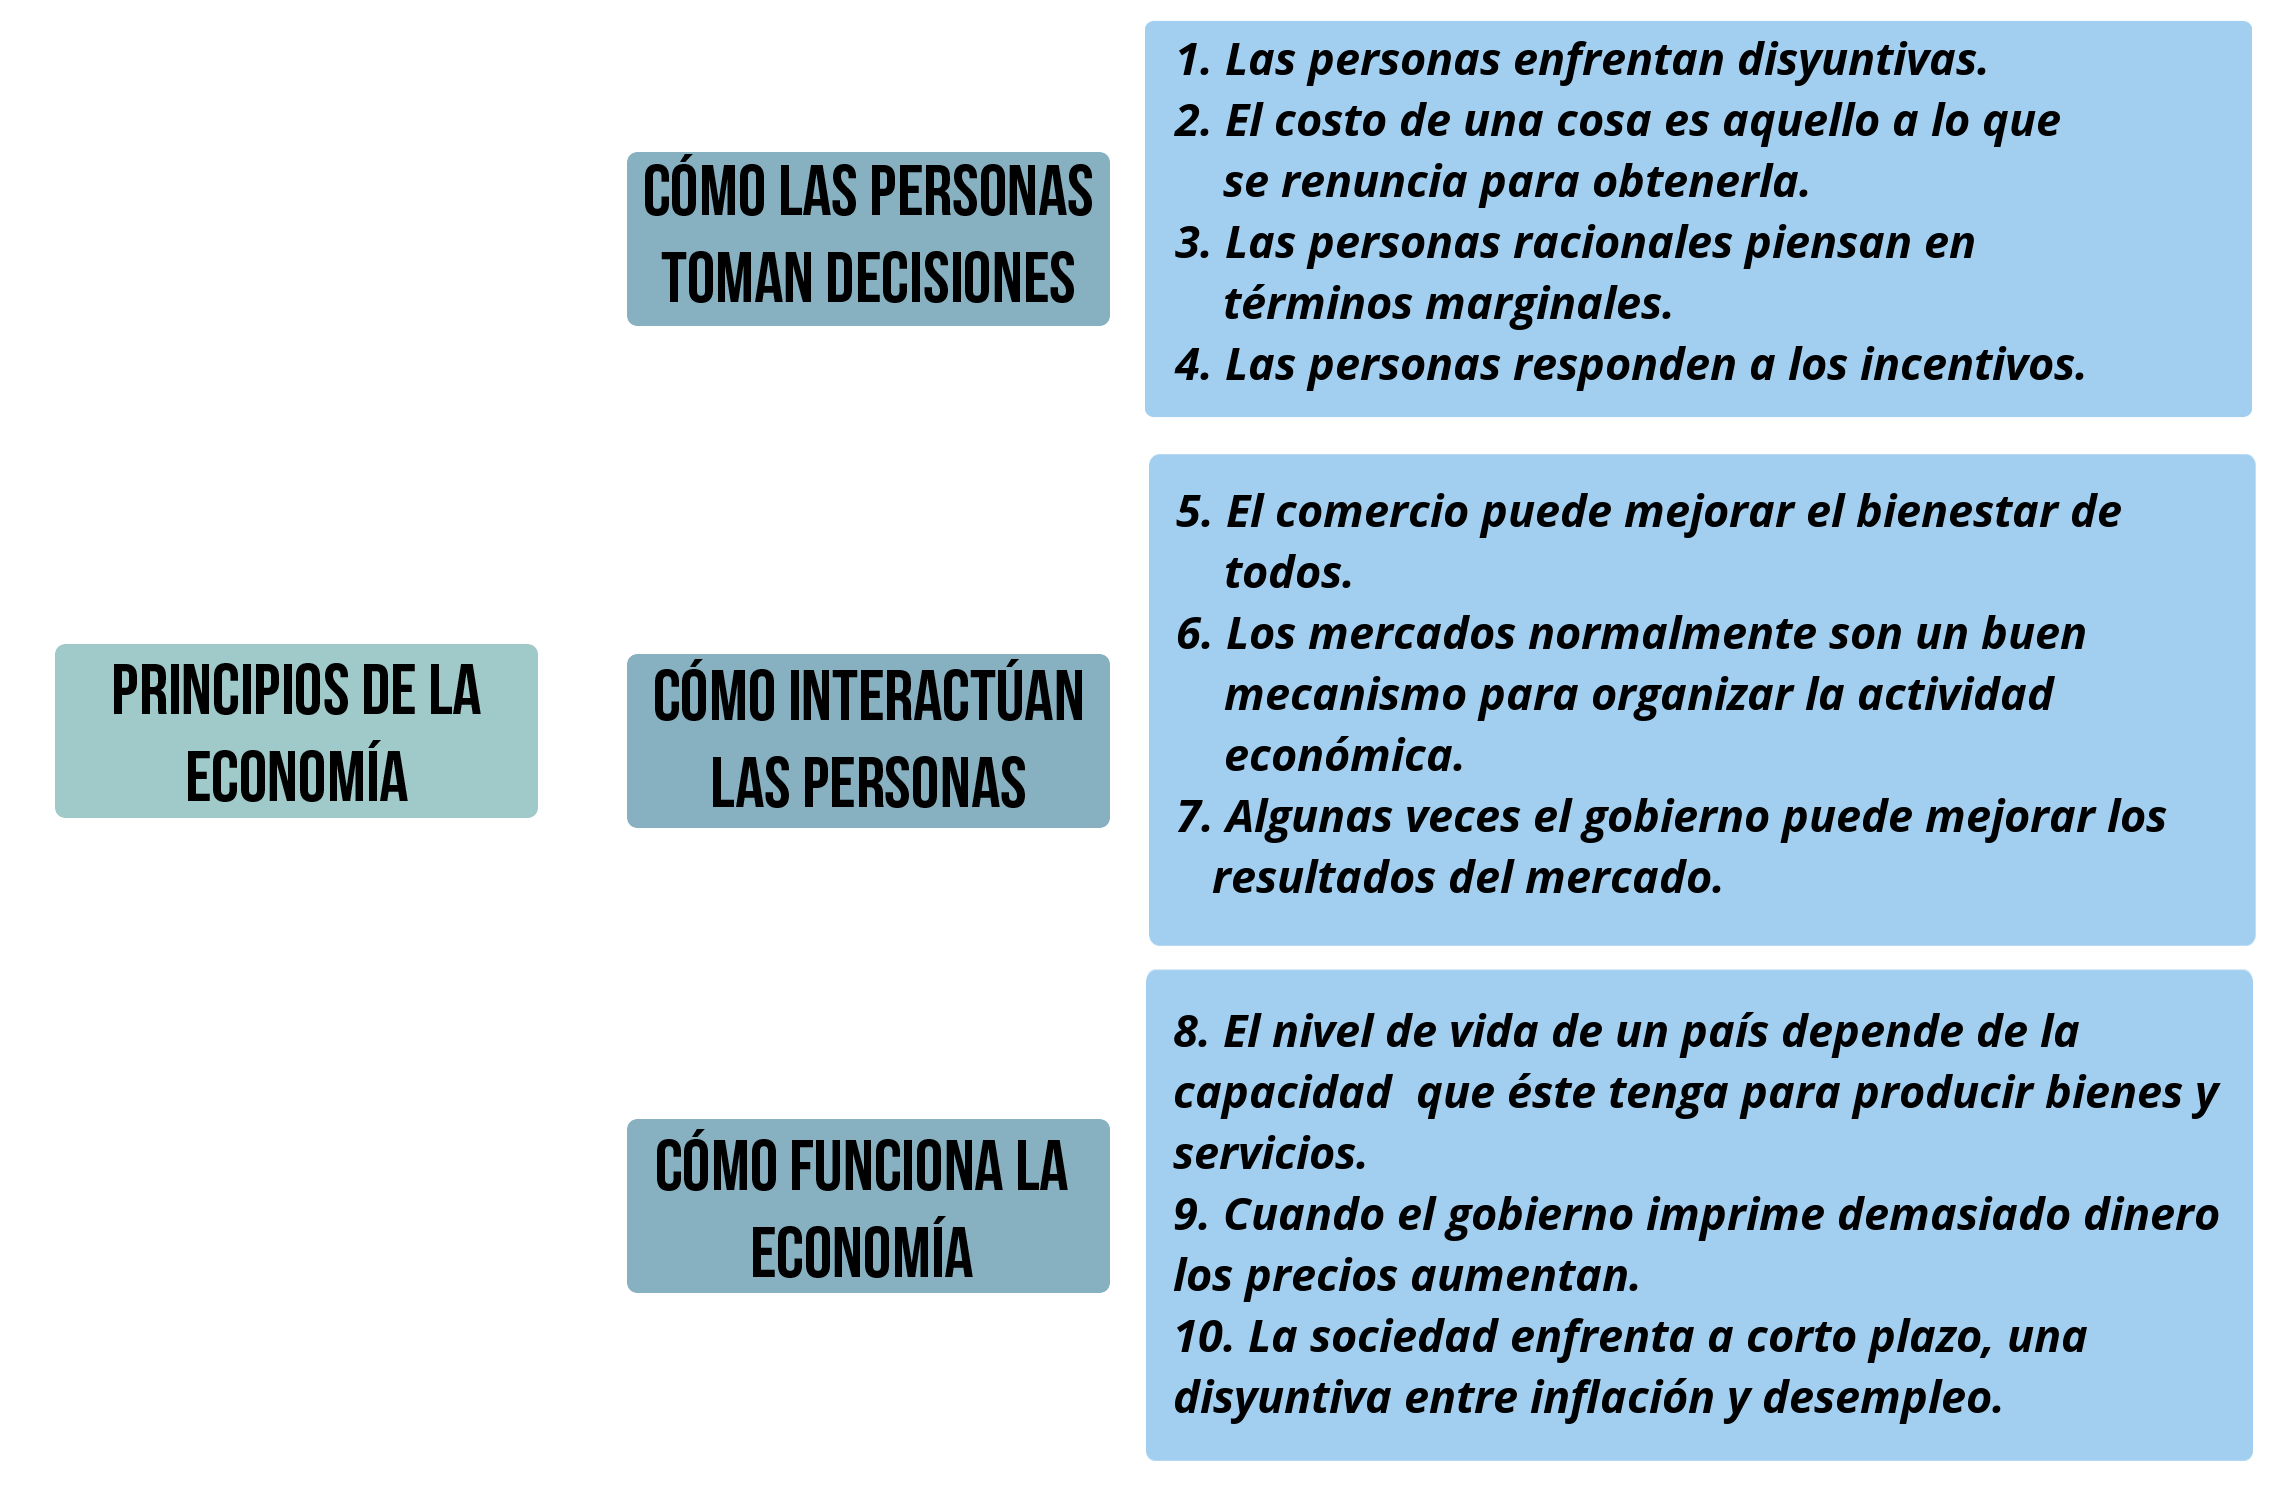
\includegraphics[width=0.65\linewidth]{images/PrincipiosEconomia}\\
\end{center}

\subsection{Cómo las personas toman decisiones.-}
Una economía no tiene nada de misterio. Independientemente de que nos refiramos
a la economía de Bolivia, a la de Estados Unidos o a la del mundo, \textbf{la economía
es solamente un grupo de personas interactuando en su vida diaria}. El comportamiento de una economía refleja el comportamiento de sus individuos, y es por esto que iniciamos el estudio de la economía con cuatro principios que regulan a los individuos al tomar decisiones.
\subsubsection{Principio 1: Las personas enfrentan disyuntivas.}
Quizá haya escuchado el dicho que asegura: \textit{"No se puede hablar y silbar al mismo tiempo".} Este dicho es muy cierto y resume la primera lección sobre toma de decisiones, \textcolor[rgb]{0,0,0.37}{ya que para obtener lo que queremos, en general tenemos que renunciar a algo que también nos gusta,} por tanto, \textcolor{azul1}{\textbf{tomar decisiones significa elegir entre dos objetivos.}} \\

La forma de actuar de la mayoría de personas implica tomar decisiones y establecer prioridades. Las disyuntivas están presentes en todos los ámbitos de la vida pero en las relaciones económicas adquieren una dimensión superior, marcando en última instancia la calidad de vida de las personas. Por ello, cualquier decisión debe tomarse ponderando si aquello que se consigue mejora aquello que se pierde o se deja de ganar.\\



Por ejemplo, si pensamos que un estudiante debe decidir cómo distribuir su recurso más valioso, es decir, su tiempo. El  estudiante puede pasar todo su tiempo estudiando matemáticas, física o dividiéndolo entre estas dos materias. Por cada hora que el estudiante destine a estudiar una materia, automáticamente dejará de estudiar la otra materia durante ese tiempo. Por cada hora que pase estudiando, automáticamente dejará de dedicar dicha hora a tomar una siesta, pasear en bicicleta, ver la
televisión o trabajar medio tiempo para así tener algo de dinero extra.\\

Ahora piense en los padres que deciden cómo gastar el ingreso familiar. Pueden comprar ropa, comida o salir de vacaciones; pueden también ahorrar una parte de su ingreso para cuando se jubilen; o bien, para pagar la educación de sus hijos. Cuando
los padres deciden gastar un dólar en uno de estos bienes, automáticamente tienen un dólar menos para gastar en otra cosa.\\

Como se expuso lineas arriba las personas toman decisiones cada día, pero también las sociedades, entendidas como el conjunto de personas, pueblos o naciones que conviven bajo normas comunes, enfrentan disyuntivas, por ejemplo una de las disyuntivas fundamentales que toda sociedad enfrenta esta dada entre la eficiencia y la equidad. La \textbf{eficiencia} significa que la sociedad extraer el máximo beneficio de sus recursos escasos. La \textbf{equidad} significa que la sociedad distribuye igualitariamente esos beneficios entre sus miembros. En otras palabras, piense en los recursos de la economía como un pastel que debe repartirse. La eficiencia sería el tamaño del pastel y la equidad la manera en cómo se reparte entre los diferentes individuos dicho pastel.\\





\subsubsection{Principio 2: El costo de una cosa es aquello a lo que se renuncia para obtenerla.}
\subsubsection{Principio 3: Las personas racionales piensan en términos marginales.}
\subsubsection{Principio 4: Las personas responden a incentivos.}